\documentclass[titlepage]{article}
%\usepackage[T1]{fontenc}
%\usepackage[utf8]{inputenc}
%\usepackage{lmodern}
%\usepackage{babel}
\usepackage{amssymb}
\usepackage{amsmath}
\usepackage[table]{xcolor}
\usepackage{booktabs}
\usepackage[hidelinks]{hyperref}
\usepackage{tabularx}
\usepackage{graphicx}
\usepackage{acronym}
\usepackage{float}
\usepackage[font=normal, labelfont = bf]{caption}
\usepackage{sidecap}
\usepackage{rotating}
\usepackage{rotfloat}
\usepackage[ampersand]{easylist}
\usepackage{multirow}

%%% page parameters
\oddsidemargin 1 cm
\textwidth 14cm
\topmargin -1 cm
\textheight 23 cm

\setcounter{tocdepth}{2}
\title{Software Project Management Plan (SPMP)}
\author{Group 2   {\em Coding Pharaohs}\\ 
\\
Abdulaziz ALHULAYFI a1642362  \\
Yu HONG	 a1616861  \\
Jianqiu LI a1635717  \\
Matthew NESTOR a1132338  \\
Yifei PEI a1611648  \\
Bowen TAO a1622211}  
\date{\today \\ Final Document}
\begin{document}
\maketitle
\tableofcontents

\pagebreak
%%REVISION HISTORY
\section{Revision History}
\begin{tabularx}\linewidth{|l|c|X|r|}
\hline
Name & Date & Reason For Changes & Version \\
\hline
Abdulaziz Alhulayfi, Yifei Pei & 6/09/2013 & Initial version & 0.1 \\
Abdulaziz Alhulayfi, Yifei Pei & 5/10/2013 & Major modifications on Risks Management and Work Plan & 1.0 \\
\hline
\end{tabularx}

\pagebreak

\listoffigures

\vspace{25pt}

\pagebreak

\listoftables


\pagebreak

%%INTRODUCTION
\section{Introduction}

%Purpose and scope

\subsection{Purpose and Scope}

%Document purpose
\subsubsection{Document Purpose and Objectives}

This \ac{spmp} describes the processes, models and schedules being followed by \ac{sep} Group 2 in their \ac{rcmr} project. This \ac{spmp} details the project's objectives, milestones and deliverables, group roles and related responsibilities, plans for risk management, a description of the group's Software Process Model, plans for configuration management, documentation, testing, and quality assurance. 

%%Intended Audience and Reading Suggestions
\subsubsection{Intended Audience and Reading Suggestions}

This document is intended for the lecturers (``clients'') of \ac{sep} Semester 2, 2013. This document is also intended for the members of Group 2 in this course, who are acting as project managers, programmers, and testers of the system. This \ac{spmp} outlines the group's approach to the project as well as specific schedules and plans that will be adhered to by all group members. 

%Project purpose
\subsubsection{Project Purpose}

The overall purpose of the project is to develop an automated ``Road Closure Marking Robot'' capable of ``mapping'' - that is, marking road closures on the roads of a ``city'' to indicate dangerous zones that are not safe to enter. \\
\\
For the purposes of this project the ``city'' is an A1-sized representation of an area that was attacked by natural disasters. ``Dangerous zones'' are the circle represented markings on the map site which illustrate the damaged areas by disasters. There are also  ``roads'' and ``obstacles'' fashioned from different representations to the map surface. The robot is required to detect these different representations on the map site. \\
\\
The group should build the system according to the client's requirements, which are gathered by the group themselves during client meetings. 

\subsubsection{Project Objectives}

The end result of the project will be to produce a robot that can detect features in the ``city'' ruins, map these features to a visual representation (an on-screen map) and a textual representation (an XML document), and mark road closures on the situations where the roads reach the dangerous zones. \\
\\
 These deliverables will be presented to the client during the final demonstration of the project in Week 13 (week beginning from 4 November 2013). 

%Project Scope
\subsubsection{Project Scope}

\label{sec:PS}
The aim of this project is to produce a prototype of an \ac{rcmr} which may be used to mark road closures and produce maps of city ruins that were attacked by natural disasters. \\
\\
This `mapping' includes producing both visual and textual representations of the site. The image-based map will be dynamically displayed on the system's \ac{gui}, while the text-based version is created and exported in the form of an \ac{xml} document.\\
\\
Within the map site, the \ac{rcmr} will detect and map only four kinds of features. These features are any roads, any obstacles, any disaster zones, and any road closures that are marked by the robot. \\
\\
Ultimately the aim is to implement the \ac{rcmr} so that it is able to mark road closures and conduct this mapping automatically.

%Assumptions and Constraints

\subsection{Assumptions and Constraints}

The assumptions that shall be considered to build the project are: 

\begin{itemize}
\item That there is a certain level of commitment from all team members
\item That all team members have a certain level of competency in at least one useful area, whether coding, writing, or project planning, etc
\item That the hardware, software and tools specified for use within the project will be suitable, reliable and relatively error-free.
\item The software shall be compatible with most of the OSs (Windows vista, 7\&8, Mac OSX and Linux)
\item The robot shall be programmed using leJOS Mindstorm
\item The machine, which will control the robot, shall have Bluetooth and USB connection devices
\item The machine, which will control the robot, shall have software for compiling and uploading code to the robot
\item The machine shall also have the java packages needed to run the program
\end{itemize}

\bigskip

\noindent The constraints that shall be considered to build the project are: 

\begin{enumerate}
\item Time
\begin{enumerate}
\item The project shall be completely delivered in one semester
\item The freezing time for the project is in week 13
\end{enumerate}
\item Resources and file sharing
\begin{enumerate}
\item The team members shall submit their files using SVN control system
\item Reused codes shall not exceed 10\% of the total project
\end{enumerate}
\item Team
\begin{enumerate}
\item The group that will develop the program shall consist of 6 members
\item The group shall have at least one group meeting a week
\item The group members will have varying degrees of competency in the various tasks required
\end{enumerate}
\end{enumerate}

\subsection{Project Deliverables}

The following table shows the project deliverables and their due dates

\newcolumntype{R}{>{\raggedleft\arraybackslash}X}%
\begin{tabularx}{\textwidth}{ l R }

Deliverable & Due Date \\
\hline
Team Poster & 12 August 2013 \\
SRS First Draft & 26 August 2013 \\
SPMP First Draft & 9 September 2013 \\
SDD First Draft & 20 September 2013 \\
Group Designated Milestone 1 & 7 October 2013 \\
Group Designated Milestone 2 & 14 October 2013 \\
Final SRS, SPMP, and SDD & 4 November 2013 \\
User Manual and Final Release of the System & 4 November 2013 \\
Testing Reports & 4 November 2013  \\
Demonstration of the System Software & Monday of week 13 \\
Group milestones and related presentations & Every Monday 

\end{tabularx}


\subsection{Evolution of the Plan}

The first draft of this \ac{spmp} is produced for submission to the client on Monday 9 September 2013. The final version of this SPMP will be submitted on Monday 4 November 2013.\\
\\
Prospective changes to the document must be raised and approved by all the group members. Once approved, changes to the written document will be made by either Yifei Pei, Project Manager, or Abdulaziz Alhulayfi, Documentation Manager.\\
\\
Changes made will be summarised in Section 1: Revision History.

\newpage

%%References
\renewcommand* {\refname}{}
\section{References}

\begin{thebibliography}{}
\bibitem{1}  Alhulayfi, A \& others 2012, ‘Project Requirements Specifications: Developing A Website for A SALeather Co’, Flinders University.

\bibitem{2} ISTQB GUIDE 2013, ‘What is Waterfall model- advantages, disadvantages and when to use it?’
\url {HTTP://ISTQBEXAMCERTIFICATION.COM/WHAT-IS-WATERFALL-MODEL-ADVANTAGES-DISADVANTAGES-AND-WHEN-TO-USE-IT/.}

\bibitem{3} Sheng, M 2013, ‘Lecture slides: Software Engineering Process Models’, University of Adelaide. 

\bibitem{4} Gantt Chart Tool 2011, Free project scheduling and management, available from: \url {http://www.ganttproject.biz/}

\bibitem{5} Timesheets 2013, the description of the usage of timesheets on forum, available from: \url {http://forums.cs.adelaide.edu.au/mod/forum/discuss.php?d=27082}

\end{thebibliography}

\newpage

\section{Definitions}

%%Acronym Definitions
%%(ref: http://ctan.unsw.edu.au/macros/latex/contrib/acronym/acronym.pdf)

\begin{acronym} 
\acro{api}[API]{Application Programming Interface}
\acro{cp}[Coding Pharaohs]{The software developing team undertaking the project} 
\acro{dtd}[DTD]{Document Type Definition}
\acro{gui}[GUI]{Graphical User Interface}
\acro{jvm}[JVM]{Java Virtual Machine}
\acro{pin}[PIN] {Personal Identification Number}
\acro{rcmr}[RCMR] {Road Closure Marking Robot}
\acro{sdd}[SDD]{Software Design Document}
\acro{sep}[SEP]{Software Engineering and Project}
\acro{spmp}[SPMP]{Software Project Management Plan}
\acro{srs}[SRS]{Software Requirements Specification}
\acro{svn}[SVN]{Subversion}
\acro{tbd}[TBD]{To Be Determined}
\acro{xml}[XML]{Extensible Mark-up Language} used to store map information

\end{acronym}

\newpage

%%PROJECT main body

%%PROJECT ORGANISATION
\section{Project Organisation}

\begin{center}
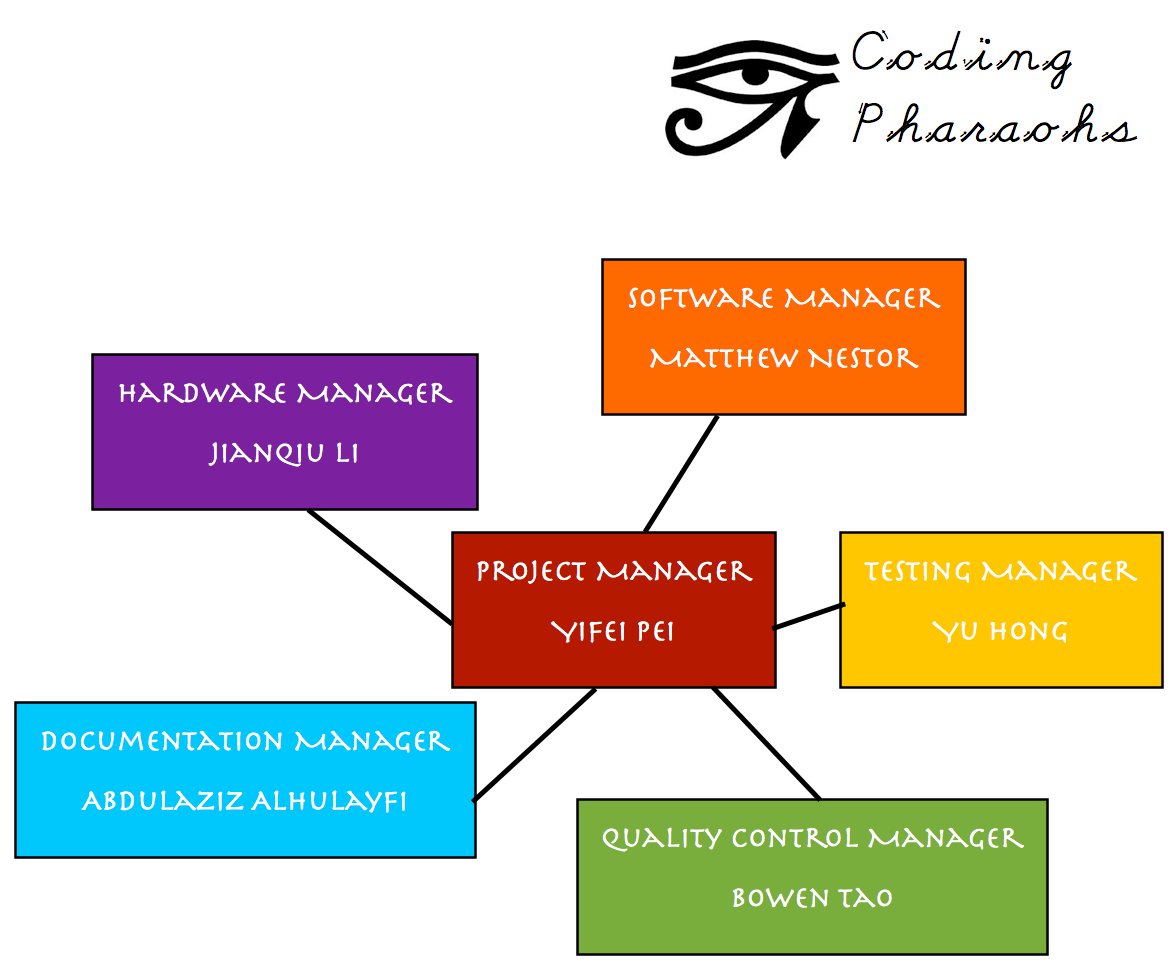
\includegraphics[scale=0.5]{images/organisation_roles.png}
\end{center}
\begin{center}
\item {Diagram 1: Organisation Chart of Coding Pharaohs}
\end{center}

%%Roles & Responsibilities
\subsection{Roles and Responsibilities}
\label{sub:roles}

Members of the group are given certain roles and responsibilities according to their specialties and where they have the high level of skills. The reason behind that is to guarantee a quality project and fair distribution between the members. However, it is required from each member of the team to contribute in every major task of the project. \\
\\
The group is divided into six roles, each of which is responsible for a particular aspect of the project. These roles are the Software Manager, Hardware Manager, Quality Control Manager, Documentation Manager, Testing Manager, and Project Manager.\\
\\
The responsibilities of each role and the group member in that role are as follows:\\
\\
\\
{\bf Project Manager: Yifei Pei}\\
\\
The project manager is in charge of the successful planning, execution, monitoring and control of the project. He shall also ensure fair contributions of all team members and make sure deadlines of project milestones are met and on time. In addition, the project manager shall ensure that project objectives and deliverables are fully defined, documented, supported and agreed by the team members. He should produce the certain outcomes for risk management and production of the SPMP. \\
\\
{\bf Software Manager: Mattew Nestor}\\
\\
The software manager is in charge of the overall performance of the software related aspects. He also shall be responsible for the general programs uploading and leJOS firmware. The software manager shall be able to assign different software tasks to team members according to their skills. Another important responsibility for the software manager is to develop the general design of the system and it’s architecture. He should produce certain outcomes for system models, UML diagrams, and production of the SDD. \\
\\
{\bf Hardware Manager: Jianqiu Li}\\
\\
The hardware manager acts as two roles since the task of protecting hardware is not a heavy workload. The hardware manager’s role in the project is to ensure all tools required for the project are provided and functioning properly. Moreover, the hardware manager shall be in charge of the robot assembly and storage. He shall keep all hardware and tools in the safety lockers that are provided by the school. The other role for the hardware manager is requirement manager. To act as a requirement manager, he is responsible for determining the requirements of the system to be built, and for specifying these in a form that can be used by the team in their production of the system. He should produce certain outcomes of the robot prototype and production of the SRS.\\
\\
{\bf Quality Control Manager: Bowen Tao}\\
\\
The quality control manager shall be responsible for setting quality standards for the whole project, making sure the standards are met, and all the outcomes are generated within the budget (time constraint).  He should ensure that the robot meets all safety, security, mission and business critical requirements. Additionally he is responsible for devising and implementing strategies for overall device security. Configuration management is another concern for quality control manager. \\
\\
{\bf Testing Manager: Yu Hong}\\
\\
The testing manager is in charge of the overall testing of each programing task to ensure errorless codes. Testing manager shall also be able to allocate testing tasks to other members accordingly. His tasks include determining and defining the scope of the tests, planning for test schedule, implementing and improving appropriate test measurements and metrics, and analysing test results and working with the team to correct any detected issues. His role is critical to make sure the group's outcomes meet the quality standards set out in SRS and SDD.\\
\\
{\bf Documentation Manager: Abdulaziz Alhulayfi}\\
\\
The documentation manager is responsible for formatting and organising all documents required for the project. He shall also be in charge of collecting the documents from other members and submitting them to the lecturers when needed. \\
\\
\pagebreak

%%RISK MANAGEMENT
\section{Risk Management Plan}
\label{sec:risk}

In a technological sense, risk can be defined as the expectation of an event’s occurrence that might affect the system in a negative way. Therefore to avoid or at least manage these risks, our team has constructed a risk management plan that defines 6 types of risks: 

\begin{enumerate}
\item Technology risks
\item Tool risks
\item Team risks
\item Requirement risks
\item Organizational risks
\item Estimation risks
\end{enumerate}

\noindent The risk management plan shall have four characters and they are as follows: \\

\begin{easylist}[itemize]
& Description: Risk details
& Probability: The likelihood of the risk to happen
&& Three levels: Low/Moderate/High 
& Effect: The possible level of effect that the risk shall do to the system. 
&& Four levels: Tolerable/Moderate/Serious/Catastrophic 
& Strategy: The steps that the group shall follow to avoid the occurrence of that risk
& Risk Indicator: The circumstances which might lead to the occurence of the risk. This helps monitoring and managing risks.
\end{easylist}

%Risks: Technology

\begin{sidewaystable}[H]

\begin{tabularx}\linewidth{|l|X|X|l|l|X|X|}
\hline
\multicolumn{7}{|c|}{Technology Risks}  \\
\hline
\#  &  Possible Risks & Description & Probability & Effect & Strategy & Risk Indicator \\
\hline
1 & Problems using new technology & There may be new technologies to some of the group members and these technologies are very important to use in the various phases of the project. Examples that can involve new technologies are: communicating with devices, learning new protocols, working with leJOS software, uploading programs etc. & moderate & catastrophic & The team shall begin working with robot and associated tools as soon as possible. Moreover, the team shall be familiar with how the devices can be connected. & \begin{itemize}
\item The group is having problems to start the project and get the robot moving.
\end{itemize}
\\

\hline
2 & Device does not function properly or is damaged & It is very necessary for the project success to have devices working properly and undamaged. Otherwise, there could be inconvenient delays, which will affect the team progressing. & low & serious & The team shall check all parts on the receipt of the kit; the team shall also take due care with equipment. In case of device damage or dysfunction, the team shall alert lecturers as soon as possible for replacement, liaise with lecturers to reschedule any missed presentations, etc.& 
\begin{itemize}
\item Delay of milestone delivery
\end{itemize}
 \\

\hline
\end{tabularx}
\caption {Technology Risks 1}
\end{sidewaystable}

\newpage

\begin{sidewaystable}[H]

\begin{tabularx}\linewidth{|l|X|X|l|l|X|X|}
\hline
\multicolumn{7}{|c|}{Technology Risks}  \\
\hline
\#  &  Possible Risks & Description & Probability & Effect & Strategy & Risk Indicator \\
\hline
3 & Software has defects & The software that shall be used for this particular project is leJOS software and it could be difficult for the group members to fix any defects due to the leJOS complexity; so this risk could be annoying for the group to do other tasks. & low & moderate & The team shall begin working with robot and associated tools as soon as possible. The team shall also program according the requirements given and familiarise themselves with the software. & 
\begin{itemize}
\item The group is having problems to compile the program.
\item Delay of milestone delivery.
\end{itemize}
\\
\hline
\end{tabularx}
\caption {Technology Risks 2}
\end{sidewaystable}

\newpage

%Risks: Tools
\begin{sidewaystable}[H]

\begin{tabularx}\linewidth{|l|X|X|l|l|X|X|}
\hline
\multicolumn{7}{|c|}{Tool Risks}  \\
\hline
\# & Possible Risks & Description & Probability & Effect & Strategy & Risk Indicator  \\
\hline
4 & Necessary tools are not provided & The project requires a number of useful tools and they critical to some phases of the project, so by not providing these tools the team could struggle in completing the project as expected in terms of time and quality. & low & serious & The team shall make sure the necessary tools for the project are provided and functioning properly. The team shall make sure the tools required for the project have been specified. & 
\begin{itemize}
\item Deliviring incomplete tasks.
\item Delay of milestone delivery.
\end{itemize}
\\
\hline
5 & Improper/ poor use of tools & The project could be affected negatively if one or more members use the required tools improperly or use it in unprofessional way.  & moderate & serious & Each team member shall immediately begin researching and using the required tools. If the team faces in difficulties, members shall seek assistance from someone proficient in using the tools. & 
\begin{itemize}
\item Deliviring incomplete tasks.
\item Delay of milestone delivery.
\end{itemize}
\\
\hline
6 & Crash of SVN server & The tool that is used to submitt documents, files and codes..etc is SVN, so the crash of SVN server will be devastating for the project progressing specially when the crash happen just before the due date & low/moderate & serious/catastrophic & The group manager shall immediately contact the topic coordinator or the IT support team in the school. & 
\begin{itemize}
\item Delay of the overall project delivery.
\item Delay of milestone delivery.
\item Deliviring incomplete tasks.
\end{itemize}
\\
\hline
7 & Bluetooth/Radio frequency errors & For this particular project, Bluetooth connection is the required method to connect the robot with the PC, so errors regarding this aspect could delay a few communication tasks.  & moderate & tolerable & The team shall perform sufficient tests before every demonstration until connection becomes efficient. & 
\begin{itemize}
\item Problems connecting the devices with each other.
\item Delay of milestone delivery.
\end{itemize}
\\
\hline
\end{tabularx}
\caption {Tool Risks}
\end{sidewaystable}

\newpage
%Risks: Team
\begin{sidewaystable}[H]

\begin{tabularx}\linewidth{|l|X|X|l|l|X|X|}
\hline
\multicolumn{7}{|c|}{Team Risks}  \\
\hline
\# & Possible Risks & Description & Probability & Effect & Strategy & Risk Indicator \\
\hline
8 & Loss of team members & The current group consists of 6 members, and losing one of them after starting the project could be a serious issue, as this would enforce the rest of the team to reallocate tasks between them, which could affect the project progressing. & low & serious &  The team shall keep frequent communications within the group. The team shall also insure all group members are always informed about others' roles and tasks. & 
\begin{itemize}
\item Redivision of tasks between group's members.
\item Deliviring incomplete tasks.
\item Delay of milestone delivery.
\end{itemize}
\\
\hline
9 & Sickness of team members & Sickness is expected to happen any time and for some type of sicknesses it could be hard for the sick member to complete tasks or contribute in tasks as expected. As a result, delays are usually expected in this situation. & moderate & moderate & The team shall keep frequent communications within the group. The team shall also insure all group members are always informed about others' roles and tasks. The team manager shall also ask whether any member can cover the sick member’s part. & 
\begin{itemize}
\item Redivision of tasks between group's members.
\item Deliviring incomplete tasks.
\item Delay of milestone delivery.
\end{itemize}
\\
\hline
10 & Conflicts between team members & It is always difficult to contribute in a group that has conflicts between members. These disagreements could make project deliverables unsuccessful or difficult. Moreover, conflicts often affect the quality of the project in a negative way. & moderate & serious & The project manager shall ensure roles and responsibilities are well defined; transparency, discussion and open decision- making shall be applied. The team manager shall make sure each area has one manager to arbitrate. & 
\begin{itemize}
\item Redivision of tasks between group's members.
\item Deliviring incomplete tasks.
\item Delay of milestone delivery.
\end{itemize}
\\
\hline
\end{tabularx}
\caption {Team Risks 1}
\end{sidewaystable}

\newpage

\begin{sidewaystable}[H]

\begin{tabularx}\linewidth{|l|X|X|l|l|X|X|}
\hline
\multicolumn{7}{|c|}{Team Risks}  \\
\hline
\# & Possible Risks & Description & Probability & Effect & Strategy & Risk Indicator \\
\hline
11 & Member does not contribute & Team members are required to contribute in each part of the project or as allocated to each member. Member not contributing in the project is a rare case however if that happened, it is usually a serious issue that affects the progress of the project in the aspects of time and quality. & low & serious &	The group manager shall guarantee fair distribution of roles and tasks according to skills and strengths. The group manager shall also ensure all members are meeting responsibilities. & 
\begin{itemize}
\item Conflicts between group's members.
\item Redivision of tasks between group's members.
\item Deliviring incomplete tasks.
\item Delay of milestone delivery.
\end{itemize}
\\
\hline
12 & Cultural/Language difficulties & It is a very common situation especially in a multicultural environment to find difficulties understanding each other ideas because of language and culture. Although it’s no one’s fault but this could cause misunderstandings.  & high & tolerable & Each member shall not hesitate to ask if there is any inconvenience and the spirit of apology shall always be present. & 
\begin{itemize}
\item Misunderstanding each other's ideas.
\item Deliviring wrong or incomplete tasks.
\item Delay of milestone delivery.
\end{itemize}
\\
\hline
\end{tabularx}
\caption {Team Risks 2}
\end{sidewaystable}

\newpage

%Risks: Requirements
\begin{sidewaystable}[H]

\begin{tabularx}\linewidth{|l|X|X|l|l|X|X|}
\hline
\multicolumn{7}{|c|}{Requirement Risks}  \\
\hline
\# & Possible Risks & Description & Probability & Effect & Strategy & Risk Indicator \\
\hline
13 & Client changes requirements & As the project is being built, the client could come up with new ideas that require changes to some of the systems’ features; therefore, this could cause certain delays of tasks and reconsiderations of the work that has been done. & low/moderate & moderate/serious & The team shall always ensure and emphasize on careful requirements elicitation; the team also shall ask for confirmation of requirements. & 
\begin{itemize}
\item Some tasks have to be redone or edited.
\item Delay of milestone delivery.
\end{itemize} 
\\
\hline
14 & Client is unavailable & Client availability is critical to the project development. For this particular project, there is a weekly client meeting in which the requirments are gathered from the client and milestones are presented by the team. So, if the client is unavailable for some reasons then there could be delys in the overall progressing of the project. & low/moderate & moderate/serious & The team shall always be prepared for such circumstances by planning alternative actions or email the client of what to do. The client shall also inform the team prior to the meeting. & 
\begin{itemize}
\item The group is working on the next milestone without insuring whether the previous milestone is met or not.
\item Delay of milestone delivery.
\end{itemize} 
\\
\hline
15 & Wrong requirements & During the first few meetings with the client, the team could misunderstand what actually the client wants due to many reasons such as the client doesn’t explain the requirements properly or the team doesn’t offer the client new ideas to help specify the requirements. & moderate & serious & The team shall always ensure and emphasize on careful requirements elicitation; the team also shall ask for confirmation of requirements. & 
\begin{itemize}
\item Some tasks have to be redone or edited.
\item Deliviring wrong or incomplete tasks.
\item Delay of milestone delivery.
\end{itemize} 
\\
\hline
\end{tabularx}
\caption {Requirement Risks 1}
\end{sidewaystable}

\newpage

\begin{sidewaystable}[H]

\begin{tabularx}\linewidth{|l|X|X|l|l|X|X|}
\hline
\multicolumn{7}{|c|}{Requirement Risks}  \\
\hline
\# & Possible Risks & Description & Probability & Effect & Strategy & Risk Indicator \\
\hline
16 & Requirements not met & The risk of missing to meet certain requirements could affect the project’s quality if not the whole project to be delivered. This risk has two scenarios and both of them could be really embarrassing for the team. The first case scenario is when the client discovers a requirement is not met when delivering the milestone and that will not be satisfactory. The second and the worst-case scenario is when delivering the final project with requirements missing which will seriously affect the project quality. & moderate & serious & The group shall ensure all requirements are met when delivering each milestone. Also each member of the team shall remind the other whether there is any requirement missing to guarantee project success and client’s satisfaction. & 
\begin{itemize}
\item Some tasks have to be redone or edited.
\item Deliviring wrong or incomplete tasks.
\item Deliviring bad quality features.
\item Delay of milestone delivery.
\end{itemize} 
\\
\hline
\end{tabularx}
\caption {Requirement Risks 2}
\end{sidewaystable}

\newpage

%Risks: Organisation
\begin{sidewaystable}[H]

\begin{tabularx}\linewidth{|l|X|X|l|l|X|X|}
\hline
\multicolumn{7}{|c|}{Organisation Risks}  \\
\hline
\# & Possible Risks & Description & Probability & Effect & Strategy & Risk Indicator \\
\hline
17 & Poor system design/ architecture & There could a risk of constructing a bad system design or architecture; and as the team progresses further some of these flaws in the design could be noticeable, thus it will be too late for effective restructuring. & moderate & serious & The whole team shall make early discussion regarding system design, iterative process whereby changes can be incrementally made; modularity to order system and keep potential contained. & 
\begin{itemize}
\item Difficulties to complete certain tasks.
\item The group constantly changes certain coding tasks.
\item Deliviring bad quality features.
\item Delay of milestone delivery.
\end{itemize} 
\\
\hline
18 & Code not up to standard & Unorganised and incorrect codes could confuse and slow down other team members. These mistakes could also affect other related codes, as they are dependent on each other. & moderate & serious & The group shall ensure careful testing regime, coding in pairs, peer review, and clear Software Quality Attributes. & 
\begin{itemize}
\item Codes are difficult to understand.
\item Program is constructed in unorgnised way.
\item Delay of deliviring certain coding tasks.
\end{itemize} 
\\
\hline
19 & No lab space & Most of the group meetings and contributed work are held in the computer lab, so it will be a waste of time to wait for a space to be available and this could also result in delay of some tasks & low & moderate & The group shall not relay only on the computers in the labs and shall try to find alternative places to work in. & 
\begin{itemize}
\item Delay of deliviring certain tasks.
\item The group is waiting for space availability outside the lab.
\item Certain tasks have noot tested on the robot.
\end{itemize} 
\\
\hline
\end{tabularx}
\caption {Organisation Risks}
\end{sidewaystable}

\newpage
%Risks: Estimation
\begin{sidewaystable}[H]

\begin{tabularx}\linewidth{|l|X|X|l|l|X|X|}
\hline
\multicolumn{7}{|c|}{Estimation Risks}  \\
\hline
\# & Possible Risks & Description & Probability & Effect & Strategy & Risk Indicator \\
\hline
20 & Underestimated time & Each phase of the project needs a fair and enough time to be completed. It is usually a huge mistake not to take tasks seriously and this could lead the team to fail delivering the project on time. & moderate & catastrophic & The team shall give and strictly follow a detailed breakdown of all tasks. The team shall be able to revise scheduling, redistribute tasks and renegotiate milestones. & 
\begin{itemize}
\item Group is late in deliviring tasks on time.
\item Deliviring bad quality features.
\item Delay of milestone delivery.
\end{itemize} 
\\
\hline
21 & Overestimate group skills/ productivity & Overestimating other members’ skills levels and productivity could be enough to make the team completely relaxed in regards to some important tasks in the project. It could also slow down the team’s progressing as well as delays delivering the milestones. & moderate & moderate & The team shall ensure and aim to modest goals; the team should be serious and careful regarding consideration of milestones and deliverables. & 
\begin{itemize}
\item Group is late in deliviring tasks on time.
\item Deliviring bad quality features.
\item Delay of milestone delivery.
\end{itemize} 
\\
\hline
22 & Missing deadlines & Delivering each milestone on time is a very critical part of the project success. If the team does not consider this risk, the team members could find themselves in a rush situation to catch up with the accumulated tasks, thus the project is very likely to be unsatisfactory. & moderate & serious & The team shall follow the project schedule which includes all due dates; major tasks and deliverables divided into smaller deliverables with evenly distributed due dates. & 
\begin{itemize}
\item Difficulties to complete certain tasks.
\item Deliviring bad quality system features.
\item Delay of milestone delivery.
\end{itemize} 
\\
\hline
\end{tabularx}
\caption {Estimation Risks}
\end{sidewaystable}

\pagebreak

%%PROCESS MODEL
\section{Software Process Model}

The process model that has been adopted for this particular project is Waterfall model. The Waterfall requires each stage of the project to be totally completed before starting the next stage of the project, after each stage the team can review what has been done for that stage to ensure the project is on the right path. The following diagram shows how the waterfall model works: \\
\\
\begin{figure}[H]
\hspace{1cm}
\vspace{0.6cm}
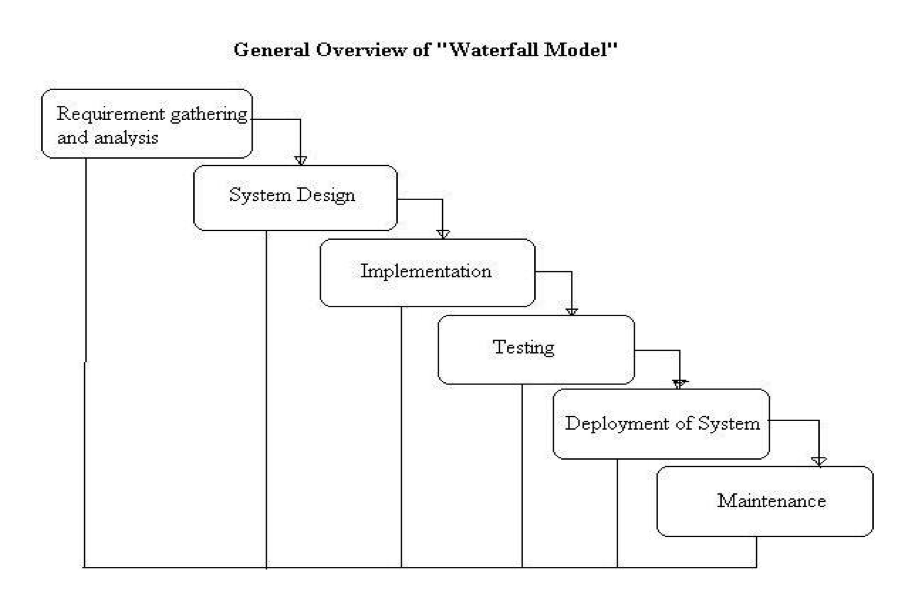
\includegraphics[width=14cm]{images/waterfall.png}
\caption {Waterfall Process Model\cite{2}}
\label{fig:waterfall}
\end{figure}

\vspace{0.75cm}

\noindent There are reasons why the team decided to choose the waterfall model and they are as follows: 
\begin{itemize}
\item Simple and easy to understand and use.
\item Easy to manage due to the rigidity of the model: each stage has specific deliverables and a review process.
\item Project stages are processed and completed one at a time.
\item Works well for smaller projects where requirements are very well understood.
\end{itemize}

\pagebreak

%WORK PLAN
\section{Work Plan}

%Work Activities
\subsection{Work Activities}
\label{sec:activities}
The acticities to deliver the project's final product can be broadly divided into two sections, the actual {\bf software development} and its accompanying {\bf documentation}.\\
\\
The activities for the development of the software can be split into Project Initiating, Requirements Collection, System Design, Implementation and Unit Testing, and Integration and System Testing. \\
\\
The activities for the development of the documentation have already been divided according to the five final documents that are required, which are the SRS, the SPMP, the SDD, the User Manual and the Testing Reports.\\
\\
The Documentation activities will run in parallel to the software development processes, with there being obvious relationships and dependencies between them: for instance, the SRS capturing the requirements ascertained during the Requirements Collection phase. Furthermore, SDD laying out the results of the System Design phase and then being used by the team to instruct the Implementation phase.\\
\\
The timelines for each phase were predetermined to an extent by the course schedule, which specified periods of requirements gathering, project demonstrations, and deadlines for the related documents. \\
\\
Additionally, other activities comprising required parts of the course should also be taken, such as the host of client meetings and the operation of meeting agendas and minutes.\\
\\
The activities involved in each of these phases are expanded upon in the following sections.\\

\begin{enumerate}

%%STAGE: Project Initiating
\item {\bf Project Initiating}\\
Week: 3\\
Duration: One week\\
\\
This phse involves all team members gaining understandings of the project as a whole, and determining the broad phases that will be required to deliver a completed product.\\
\\Activities include:
\begin{enumerate}
\item Read and understand Project Description
\item Start to learn tools and knowledge required to complete the project and specific skills for different roles
\item Basic scheduling: broad weekly overview
\item Get understandings of different roles and determine responsibilities accordingly \\
\end{enumerate}
Concurrent Documentation: SPMP. Activities include:
\begin{enumerate}
\item Defining tasks in order to deliver the finished product: Work Activities
\item Allocating tasks to different roles: Position Descriptions
\item Devising an initial schedule for all the tasks, taking into account related deadlines: Schedule Allocation
\item Writing introductory material \\
\end{enumerate}

%%Stage: Requirements Collection
\item {\bf Requirements Collection}\\
Weeks: 3 - 5\\
Duration: Three weeks\\
Determined by: The Client Meetings of Weeks 3 \& 4 are specifically for Requirements elicitation; First Draft of SRS due on Monday 26 August (Monday Week 5).\\

This phase involves expanding on the initial Project Description to determine the client's needs in detail. The elicited requirements are then used to construct the Software Requirements Specification document.\\
\\Activities include:
\begin{enumerate}
\item Determining areas and details that need clarification from the original specification (Project Description on Course Website)
\item Formulate questions to ask the client
\item Question client during two scheduled Requirements Elicitation meetings\\
\end{enumerate}
Concurrent Documentation: SRS. Activities include:
\begin{enumerate}
\item Collating gathered information into discrete, well-defined and specific requirements documentation
\item Define acceptance criteria for all requirements
\item Define Use Cases
\end{enumerate}

%%Stage: System Design
\item {\bf System Design}\\
Weeks: 5 - 9\\
Duration: Five weeks\\
Determined by: First Draft of SDD due on Friday 20 September (Friday Week 8).\\
Overlaps with Implementation and Unit Testing, since normally issues not realised during the design phase will emerge during implementation.\\
\\
This phase involves designing the overall architecture of the system, so that it will deliver the functionality described in SRS. The results of this design are detailed in the SDD, the first draft of which is due at the end of this design phase.\\
\\Activities include:
\begin{enumerate}
\item Defining a state diagram to illustrate how the robot will work
\item Break the design into implementable components
\item Define classes and interfaces
\item Define data stores and logic elements
\item Defining Class, State and Interaction information
\item Design the User Interface for the PC-side of the system
\end{enumerate}

Concurrent Documentation: SDD. Activities include:
\begin{enumerate}
\item Create UML diagrams: Class, State and Interaction diagrams
\end{enumerate}


%%Stage: Implementation and Unit Testing
\item {\bf Implementation and Unit Testing}\\
Weeks: Mid-semester break Weeks 1 \& 2; Weeks 9 - 12\\
Duration: Six weeks\\
Determined by: Milestones 1 due on Monday of Week 9; Milestone 2 due on Monday of Week 10; Final Presentation due on Monday of Week 13.\\
Overlaps with System Design Phase, as described in last phase.\\
\\
This phase involves coding the majority of the system, working from the design laid out in the SRS.\\
\\
This phase is broken into smaller stages of Implementation, namely:\\
\\
First Stage: Mapping under manual control (Milestone 1)\\
Second Stage: Mapping under AI mode (Milestone 2)\\
Third Stage: Integration of all features (Final Presentation)\\
\\
Due to time constraints and the fact that there are several stages of Implementation, this phase overlaps with the following Integration and System Testing phase.\\
\\First stage tasks include:
\begin{enumerate}
\item Creating a GUI with movement controls and map display area 
\item Implementing PC-robot connection via blue-tooth (connection made via GUI)
\item Implementing movements \& `behaviours' so that robot can be directed to move around map
\item Implementing mapping so that the GUI can represent the explored new areas detected by robot while navigating under manual control
\end{enumerate}

Second stage tasks include:
\begin{enumerate}
\item Implementation of disater zone and obstacle detection so that the robot stops instantly when it meets the disaster zone or obstacles
\item Implementing Path-finding algorithm so that robot can navigate map site automatically without controller intervention
\item Implementing the road closure marking function so that the robot can automatically mark road closures appropriately
\item Implementing saftey functioning of the robot so it can deal with emergency conditions
\end{enumerate}

Third stage tasks include:
\begin{enumerate}
\item Implementing a comprehensive functionality of the robot so it can integrate different development components together and perform the designated and required features
\item Review all requirements in SRS so as to guarantee that both functional and non-functional requirements have met and fulfilled in this project
\\
\end{enumerate}

Concurrent Documentation: Testing Reports; SDD, SRS. Activities include:
\begin{enumerate}
\item Each group member to define JUnit test cases to test their own code
\item Writing individual test reports
\item Collating these individual reports to overall Group Testing Report
\item Incorporating any changes to overall structure that are found to be necessary as build progresses into SDD
\item Incorporating any changes to overall functioning that are found to be necessary as build progresses into SRS
\\
\end{enumerate}


%%Stage: Integration and System Testing
\item {\bf Integration and System Testing}\\
Weeks: Mid-semester break Week 2; Weeks 9 - 12\\
Duration: Five weeks (overlaps with previous Implementation and Unit Testing phase)\\
Determined by: Milestones 1 due Monday Week 9; Milestone 2 due Monday Week 10; Final Presentation due Monday Week 13.\\
\\
This phase involves integrating individual components and testing the system as a whole to identify problems and ensure that it functions correctly.\\
\\Activities include:
\begin{enumerate}
\item Integration Tests
\item User Tests
\end{enumerate}

Concurrent Documentation: Testing Report; SDD, SRS. Activities include:
\begin{enumerate}
\item Including results from Integration Testing counting into overall Group Testing Report
\item Changes to SDD and SRS as described previously
\end{enumerate}


\end{enumerate}

\pagebreak

%Schedule allocation
\subsection{Schedule Allocation}
\label{sec:schedule}

All schedules generated in this document are planned and maintained by using the tool, GanttProject \cite{4}.\\
\\
The activity duration describes the total time that passed for that activity but not the actual undertaken time. For instance, one activity takes two hours undertaken time but the two hours working time is distributed into a two days' working section. For the situation described above, the duration of that activity is two days. The schedule was made by a project management scheduling tool and determined by the group, rather than a personal time-management tool. It is anticipated that smaller dependencies will be negotiated between team members. \\
\\
Following the ``Waterfall'' method, the broad activities, as defined in section 8.1, are scheduled to occur in a relatively consecutive fashion. ``Documentation'' occurs in parallel with all other phases throughout the schedule. This may be seen in Figure \ref{fig:overview}:\\

%Overview
\begin{figure}[H]
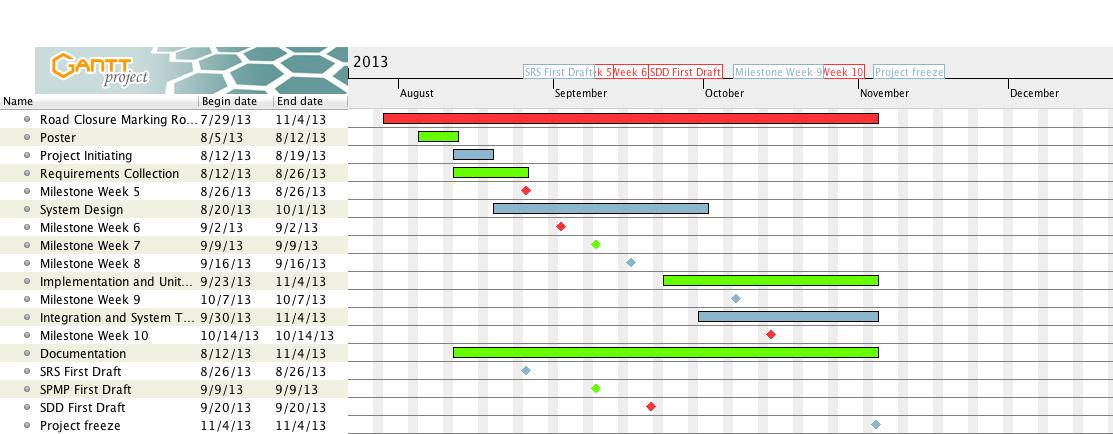
\includegraphics[width=14cm]{images/gantt/overview.jpg}
\begin{center}
\caption [Gantt chart: Schedule overview]{Gantt chart: Overview of schedule in which stages components occur consecutively. `waterfall'-like appearance.} 
\label{fig:overview}
\end{center}
\end{figure}

\noindent The followings show detailed schedules for individual phases, including {\bf Project Initiating}  in Figure \ref{fig:pi}, {\bf Requirements Collection} in Figure \ref{fig:rc}, {\bf System Design} in Figure \ref{fig:sd}, {\bf Implementation and Unit Testing} in Figure \ref{fig:iut}, {\bf Integration and System Testing} in Figure \ref{fig:ist}. Some of the pre-quisite activities and fowllowing activities that may exceed the time fram of the phases are also spotted into the relevant phases for the convenience of audience. \\

%Initiating
\begin{figure}[H]
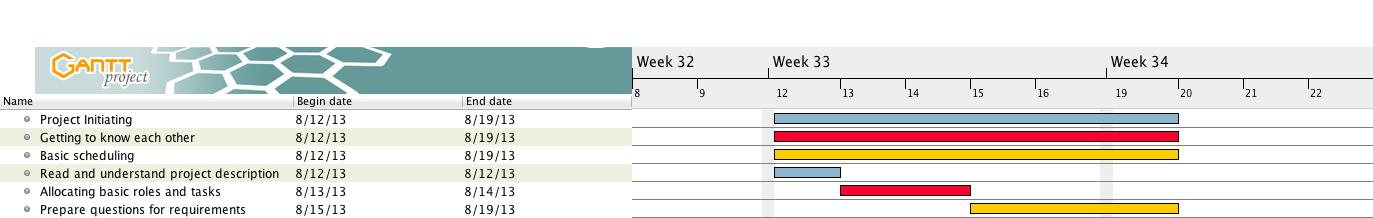
\includegraphics[width=14cm]{images/gantt/init.jpg}
\caption {Gantt chart: Project Initiating Phase}
\label{fig:pi}
\end{figure}



%Requirements Collection
\begin{figure}[H]
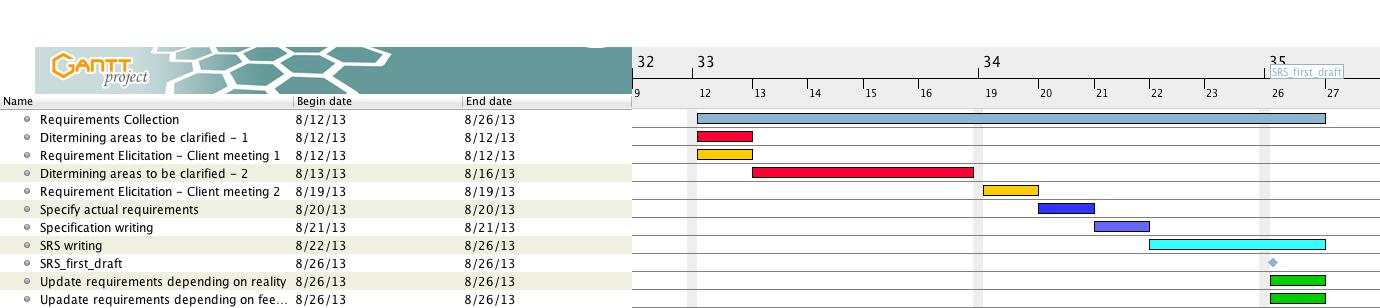
\includegraphics[width=14cm]{images/gantt/requirement.jpg}
\caption {Gantt chart: Requirements Cllection Phase}
\label{fig:rc}
\end{figure}


%System Design
\begin{figure}[H]
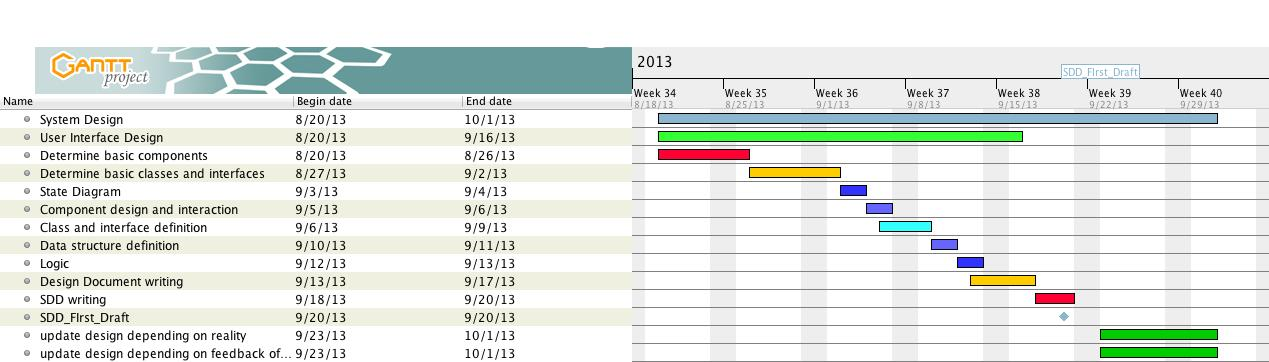
\includegraphics[width=14cm]{images/gantt/design.jpg}
\caption {Gantt chart: System Design Phase}
\label{fig:sd}
\end{figure}


%Implementation and Unit Testing
\begin{figure}[H]
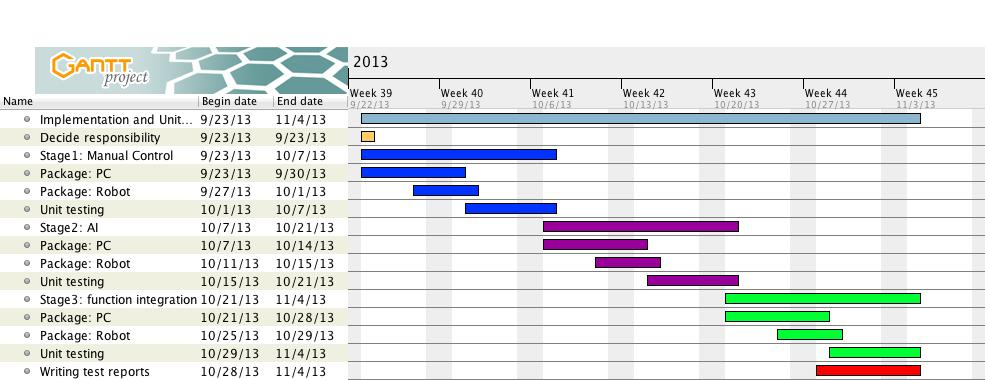
\includegraphics[width=14cm]{images/gantt/test1.jpg}
\caption {Gantt chart: Implementation and Unit Testing}
\label{fig:iut}
\end{figure}


%Integration and System Testing
\begin{figure}[H]
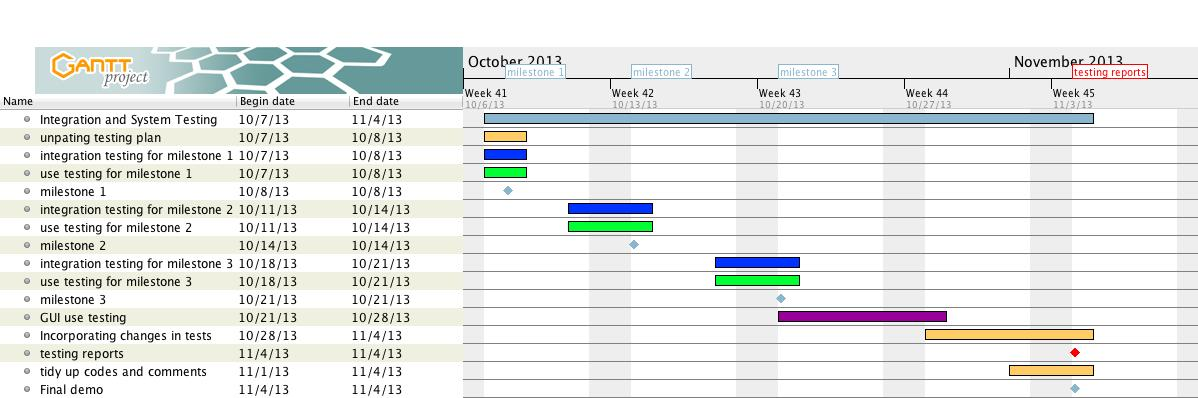
\includegraphics[width=14cm]{images/gantt/test2.jpg}
\caption{Gantt chart: Integration and System Testing}
\label{fig:ist}
\end{figure}



%detailed overview
%\begin{figure}
%\begin{sidewaysfigure}
%\vspace{-1cm}
%\hspace{-2cm}
%%%\includegraphics[scale=0.55]{images/gantts/1_Overview_detail.pdf}
%\caption[Gantt chart: Sub-components of Major phases]{Gantt chart: Schedule overview showing sub-stages of the major Software Development stages, as well as their relationship to the Documentation production schedule.}
%\label{fig:ist}
%\end{figure}
%\end{sidewaysfigure}

\pagebreak

%Resource allocation
\subsection{Resource Allocation}
As discussed in Section \ref{sub:roles}, each member of the team has been assigned a particular area of responsibility. At a given time, any group member may be more or less active, depending on the extent to which their role is involved or required for the current development phase.\\
\\
The tasks assigned to the Project Manager, Yifei Pei, are spread evenly throughout the project, with tasks of working with the various sub-Managers and tracking the regular works of the group. The Project Manager is also responsible for compiling and overseeing production of the \ac{spmp}, and he is particularly involved with the preparation of this document prior to the first draft and final version submissions.\\
\\
Matthew Nestor, as Software Manager, has primary responsibility for the design of the project's software. As such, the role is particularly involved in the production of the \acl{sdd}.\\
\\
Hardware Manager, Jianqiu Li, who is also responsible for requirements management, has the tasks of determining the requirements of the system to be built. He should work with Sofware manager to make sure that the requirements are reflected in the final system design. He is also responsible for making an apropriate robot prototype.\\
\\
The Testing manager, Yu Hong, is responsible for specifying and managing the testing tasks that are to be shared among the group. This role is more active later in the project, during the scheduled `Implementation and Unit Testing' and `Integration and User Testing' phases.\\
\\
Quality Control Manager, Bowen Tao, is responsible for setting standards for the group members to adhere to when producing documents and code, controling the outcomes of the group to meet the standards and monitoring the group work process to ensure the project is completed within constraints.\\
\\
The Documentation Manager, Abdulaziz Alhulayfi, is responsible for all documentation, both formal and informal, created as part of the project. This includes working with other sub-Managers on the major documents and maintaining the \acs{svn} repository.\\
\\
As well as allocating specific people to specific areas, all group members are responsible for writing code. Dividing and allocating the components to be written is a task of the Software Manager.

%Team member resources
%\begin{figure}[H]
\begin{sidewaysfigure}
%\vspace{0.5cm}
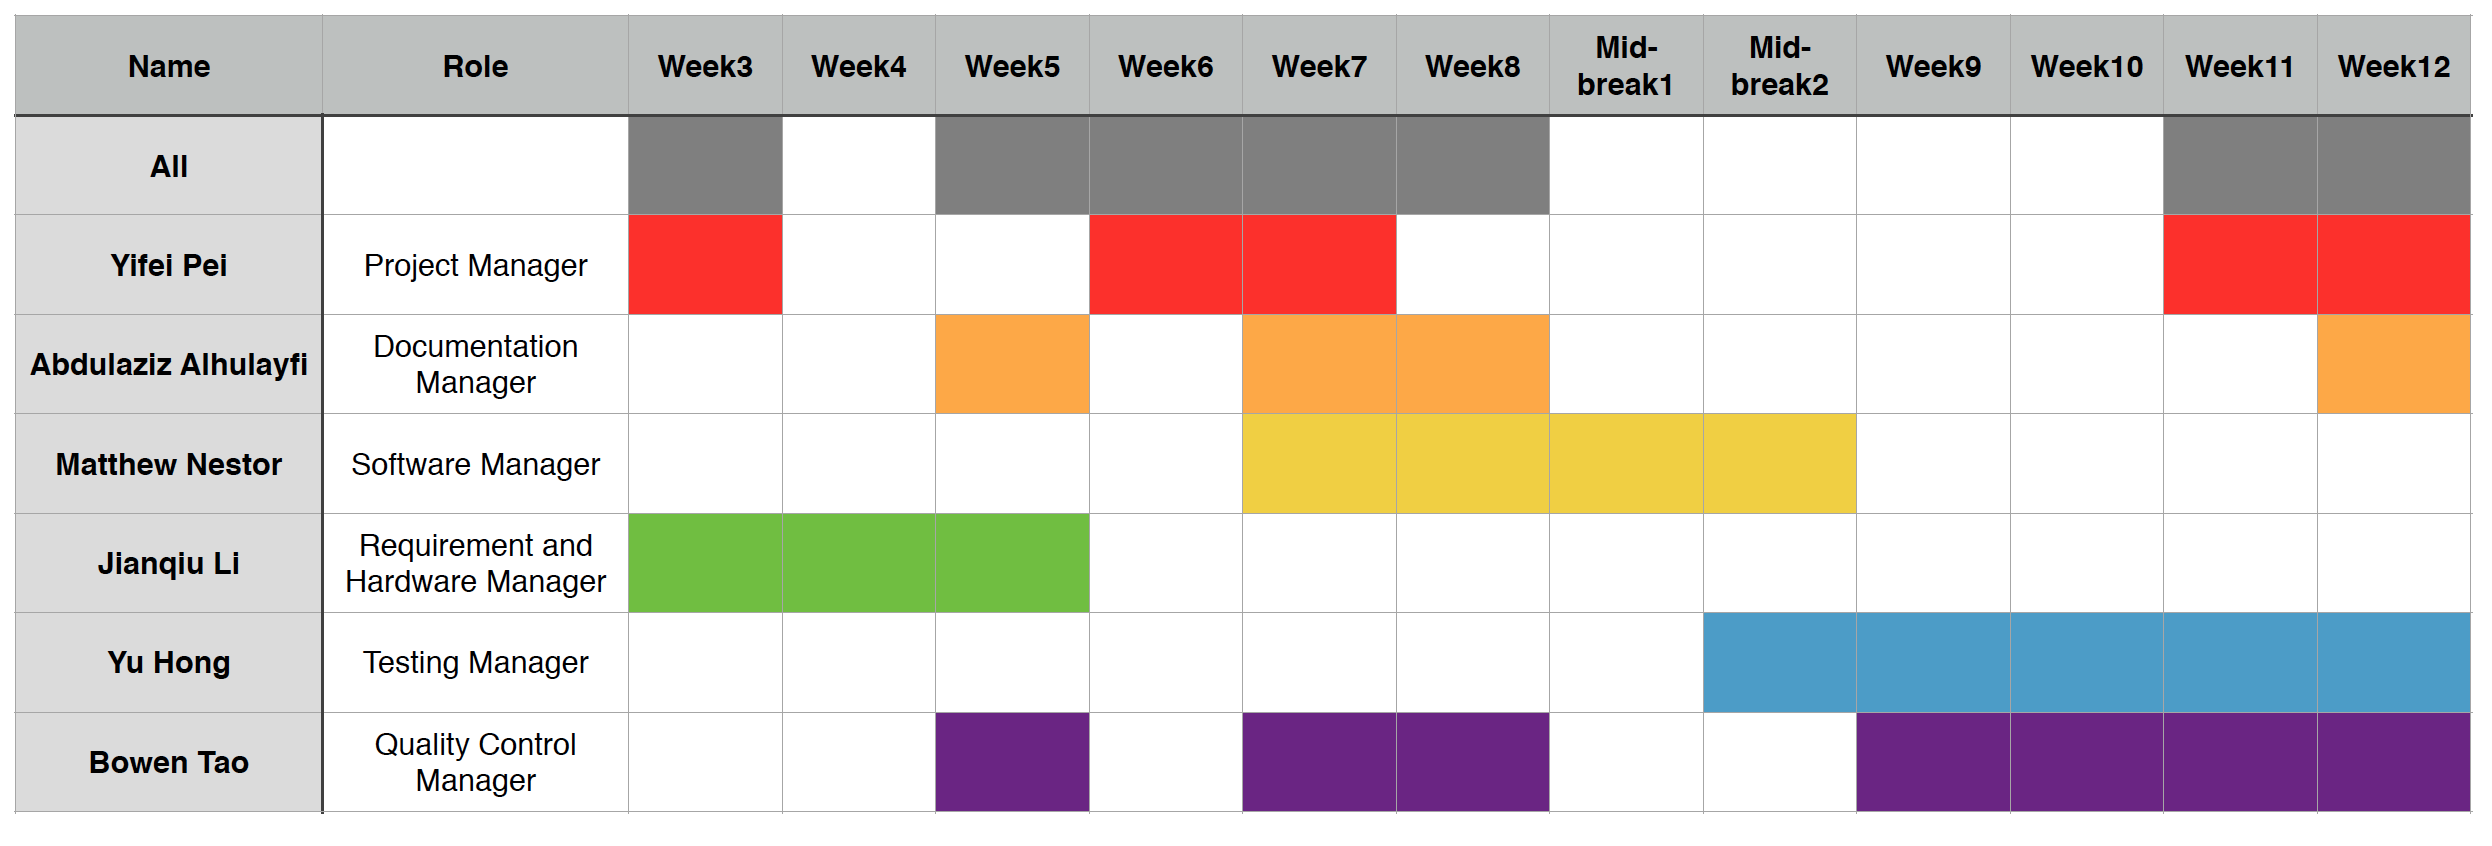
\includegraphics[width=24cm]{images/gantt/NewResources.png}
\caption[Allocation of Team Member resources across the project]{Allocation of resources (team members) across the project. Note that members who do not have any tasks assigned solely to them for a particular week may be involved in tasks allocated to `All' .}
\label{fig:r}
%\end{figure}
\end{sidewaysfigure}

\pagebreak


%MILESTONES
\subsection{Milestones}
The following Milestones list the functionality to be presented prior to the final delivery of the project.

%%Milestones 1
\subsubsection{Milestones 1: To be presented on Monday 7 October}

{\bf GUI features}

\begin{enumerate}

\item Map editor redesign

\begin{itemize}
\item The representation of the robot (indicate the facing direction)
\item Position the (0,0) point at the botom left rather than top left.
\item Larger scaled map than the previous one
\item Use tiles to present the map contents (Suggested by the client at the client meeting Week 7)

\end{itemize}

\item Real-time map generation

\begin{itemize}
\item Present the current location of the robot
\item The newly explored area and objects will be presented on the GUI in real-time
\end{itemize}

\end{enumerate}

\noindent {\bf The manual control of the robot}

\begin {enumerate}
\item The user can manually control the robot to explore the map
\item Manually road closure marking
\end {enumerate}

\noindent {\bf Safety performance}

\begin {enumerate}

\item Movement speed

\begin{itemize}
\item Provide a speed bar on the GUI to manually control the speed of the robot
\item The maximum speed should be within a safe value
\item The primary hypothesis setting for the speed is from 1cm/s to 5cm/s. This hypothesis needs further testing to verify. (It may change depending on the testing data.)
\end{itemize}

\end {enumerate}

\noindent {\bf Map site testing designed by the group}

\begin {enumerate}
\item A1 size map with basic features prepared by the group
\end {enumerate}

\pagebreak

\subsubsection{Milestones 2: To be presented on Monday 14 October} 

{\bf GUI features}

\begin {enumerate}

\item Present traversed path by the robot

\begin{itemize}
\item Use a different colour on the map to display the traversed path by the robot
\end{itemize}

\item Machanism for the robot to get to the starting position on map

\begin{itemize}
\item By clicking a button called ``set location''  to enable the ``go-to-starting-position'' mode of the robot, and click again to disable the mode after correctly set the starting position of the robot
\item Use mouse motion to drag the robot to the map (Suggested by the client at the client meeting Week 7)
\end{itemize}

\end {enumerate}

\noindent {\bf AI mode of the robot}

\begin {enumerate}
\item Automatically follow the road and explore uncleared area
\item Obstacle and disaster area avoidance
\item Automatically road closure marking
\item The robot has the ability to go back to the starting position in AI mode (Exit)
\end {enumerate}

\noindent {\bf Safety performance}

\begin {enumerate}

\item Collision detection. Once collision happens, the robot should stop immediately. 

Collisions include: 

\begin{itemize}
\item Hitting obstacles
\item Entering disaster zones
\item Off road
\item Out of map
\end{itemize}

\item Dangerous zone.

\begin{itemize}
\item The robot should never go into the dangerous zone. Once it reaches the edge of the area, it will immediately stop.
\end{itemize}

\end {enumerate}

\noindent {\bf Map site testing designed by the group}

\begin {enumerate}
\item Put obstacles on the map and test
\end {enumerate}

\pagebreak

\subsubsection{Milestones 3: To be presented on Monday 21 October} 

{\bf GUI features}

\begin {enumerate}

\item Real-time messages on GUI

\begin{itemize}
\item There will be a display field on the control panel of the GUI to show real-time messages sent by the robot.
\item The messages are going to report the status of the robot, including warnings and necessary values that the operator needs to know.
\end{itemize}

\item Zoom feature for the map

There are two designated methods to implement this feature. The group will choose the better one depending on testing data.

\begin{itemize}
\item Place a zoom bar under the map to control the size of display area on the map panel. 
\item Place a smaller full view of the map beside main display of the map panel. The main display will show a certain sized part of the map. The user can drag the rectangle indicator in the full view map or use the scrolling bar to control the display area in the main display. (Suggested by the client at the client meeting Week 4)
\end{itemize}

\end {enumerate}

\noindent {\bf Manual control mode features}

\begin {enumerate}

\item Manual mode collision detection. Once collision happens, the robot should stop immediately against any manual command from the operator. The definitions for collision have been declared in the milestone for Week 10.

\end {enumerate}

\noindent {\bf AI mode features}

\begin {enumerate}

\item If the robot is forced to stop, it has the ability to continue the uncompleted AI mode exploration once the problems are solved.

\end {enumerate}

\noindent {\bf Safety performance}

\begin {enumerate}

\item Low power performance.

\begin{itemize}
\item Send warning message to the operator when the battery has 20\% life left.
\item If the battery has only 5\% life left, the robot will immediately stop.
\end{itemize}

\item Lost of connection performance. 

\begin{itemize}
\item Stop, and once connected go to manual control mode.
\end{itemize}

\end {enumerate}

\pagebreak


%%SUPPORTING PLANS
\section{Supporting Plans}
\subsection{Configuration Management plan}

This plan specifies how document and file control as well as version control will be conducted along with the development of this project.  As the project has been segmented and allocated to different group members based on their experience and expertise, there will be frequent updates of project versions. Therefore it is vital to develop a scheme to control the processes of document editing and group collaboration.\\

\subsubsection{Version Control}

The project adopts the Subversion (SVN) version control system, which creates a group repository that can be used by all team members for sharing documents, files, code, testing scripts and useful tools. Branches are also created in the group repository so that each group member could work on their individual part of the project and update with others' work simultaneously and finally merge the whole project together. Moreover, by using SVN, version control, which includes tasks such as reverting to previous versions to find missing information or retrieving a mis-deleted file by tracking back the submission history, becomes much easier and more efficient in terms of implementing the project development requirements.\\
\\
All major documents will be attached with a version number. For the version number used by group members to modify and update, the number starts from 0.1 and climbs up in increments such as 0.1, 0.2, 0.3 and so forth. \\
\\
For the version control of codes, it will only have 3 different version numbers which are milestone 1, milestone 2 and the Final version. These versions are the stable version of the codes combined with the documentation which is ready to be released to the client at the same time. For retrieving the frequently updated code along with the progress, ``svn log'', ``svn status'' and ``svn diff'' will be used to trace the changes in the code.\\
\\
Furthermore, for major documents of this project, there will be a table list at the beginning of each document specifying the version numbers of each iteration, after the group modify the contents. Only major changes to structure or content will be allocated to a new internal version number. For minor changes such as grammar, typos, or sentence structure changes, there will be no new version numbers allocated. Those changes will be traced back from SVN committing comments.\\

\subsubsection{SVN submission}

All group members should do a SVN update before adding or deleting any item in the group repository as part of the version control plan to reduce the possibilities of version conflict.  By adopting the same submission commenting style, comments will be easily understood. Additionally, prior to every major project document submission, the submitted document will be ``tagged'', by adding a copy of the document to the `tags' directory in the repository.\\
\\

\newpage


\subsubsection{Group Repository Tree }

\begin{center}
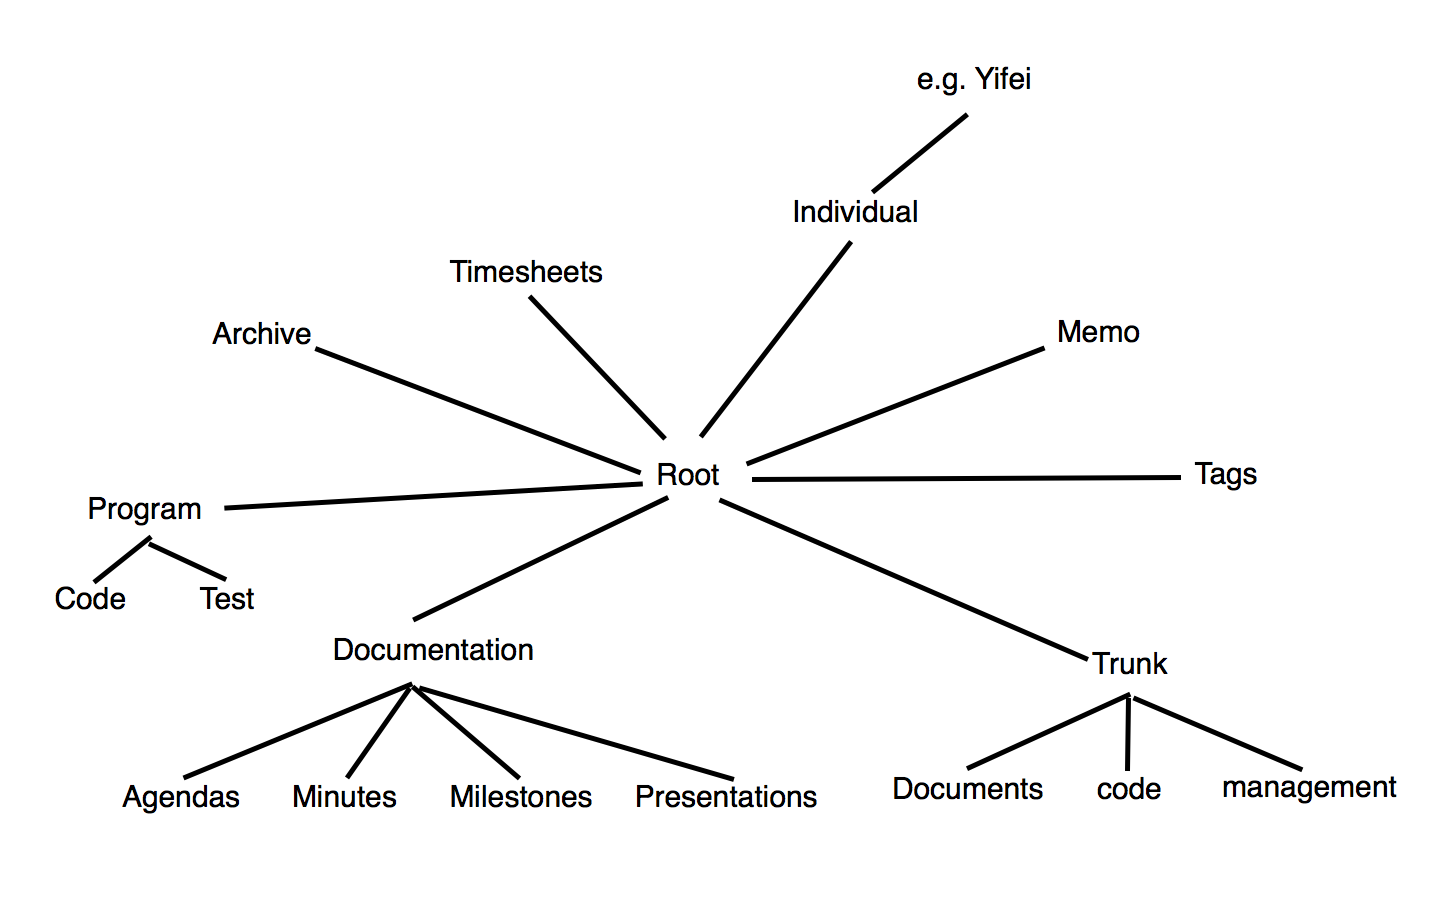
\includegraphics[scale=0.5]{images/SVN_tree.png}
\end{center}

\begin{center}
\item {Diagram 2: Group Repository}
\end{center}

\noindent {\bf Archive} \\
\\
Folder contains helping documents for group members to use as a reference, such as rules for group machanism, SVN fuctioning description, helping files for group members' better learning, working examples as well as conventions for different tools. \\
\\
{\bf Documentation} \\
\\
All the documentations should go here, including agendas and minutes for both the client meetings and group meetings, milestones' supplementary documents, and presentation supporting documents. \\
\\
{\bf Individuals} \\
\\
Individual folders for group members. One can do anything within his individual folder. \\
\\
{\bf Memo} \\
\\
Folder contains files for group members to keep tracking what he did in the past week
and what needs to do in weeks ahead. Additionally, brainstorming exercises, memos to leave short message to fellow members and communicate with each other, and anything a group member wants to remember or wants to show to the whole gorup can all be put in this folder. \\
\\
{\bf Program} \\
\\
Contains the sub folders of code and test, to store source codes of the project's system and testing files. \\
\\
{\bf Tags and Trunk} \\
\\
Tags folder is to store the final release of submitted project and documents. Trunk is a folder to generally store the files that should worked by the whole group together and submitted later. \\
\\
{\bf Timesheets} \\
\\
This folder is to store the timesheets that contain the working hours for each week of every team member. The existence of these timesheets is going to support the statistics analysis conducted by lecturers to assess the working process of different groups\cite {5}. \\

\subsection{Documentation Plan}
\subsubsection{General outline}

Each of the three major documents will be lead by a group of two to decide the content, structure and task allocation under the documentation scheme. The two people in the three document oriented groups will develop the documents within their domain knowledge over the project while supported by the rest of the team.\\

\begin{table}[H]

\begin{tabular}{|c|c|c|c|}
\hline
Assign & Deadline & Deadline for ind & Res people  \\
\hline
SRS first draft & 26 August (Week 5) & 23 August & Jianqiu, Yu \\
\hline
SPMP first draft & 9 September (Week 7) & 6 September & Aziz, Yifei \\
\hline
SDD first draft & 20 September (Week 8) & 17 September & Bowen, Matt \\
\hline
\end{tabular}
\caption {Major documentation scheme}
\end{table}

\noindent The group members will take turns to be the chair and secretary of client meetings. Generally, the chair is responsible for writing the agenda and the secretary is responsible for writing the minutes. For every client meeting, an agenda must be provided 24 hours before the meeting and a minutes must be summarised 24 hours after the meeting. Therefore the deadline for agenda is 2.30pm Sunday before the client meeting and the deadline for minutes is 2.30pm Tuesday after the client meeting. The people who are responsible for writing them are also responsible for printing them out and bringing them to the client meetings.\\


\begin{table}[H]

\begin{tabular}{|c|l|c|l|}
\hline
NO. & Time & Roles & Name \\
\hline
\multirow{2}{*}{1} & \multirow{2}{*}{2.30pm - 3.00pm 12 August} & Chair & Yifei Pei \\ 
                            &                                                                        & Secretary & Matthew Nestor \\
\hline
\multirow{2}{*}{2} & \multirow{2}{*}{2.30pm - 3.00pm 19 August} & Chair & Aziz \\ 
                            &                                                                        & Secretary & Bowen Tao \\
\hline
\multirow{2}{*}{3} & \multirow{2}{*}{2.30pm - 3.00pm 26 August} & Chair & Bowen Tao \\ 
                            &                                                                        & Secretary & Jianqiu Li \\
\hline
\multirow{2}{*}{4} & \multirow{2}{*}{2.30pm - 3.00pm 2 September} & Chair & Jianqiu Li \\ 
                            &                                                                        & Secretary & Matthew Nestor \\
\hline
\multirow{2}{*}{5} & \multirow{2}{*}{2.30pm - 3.00pm 9 September} & Chair & Matthew Nestor \\ 
                            &                                                                        & Secretary & Yifei Pei \\
\hline
\multirow{2}{*}{6} & \multirow{2}{*}{2.30pm - 3.00pm 16 September} & Chair & Yifei Pei \\ 
                            &                                                                        & Secretary & Yu Hong \\
\hline
\multirow{2}{*}{7} & \multirow{2}{*}{2.30pm - 3.00pm 7 October} & Chair & Yu Hong \\ 
                            &                                                                        & Secretary & Aziz \\
\hline
\multirow{2}{*}{8} & \multirow{2}{*}{2.30pm - 3.00pm 14 October} & Chair & Aziz \\ 
                            &                                                                        & Secretary &  Bowen Tao\\
\hline
\multirow{2}{*}{9} & \multirow{2}{*}{2.30pm - 3.00pm 21 October} & Chair & Yu Hong \\ 
                            &                                                                        & Secretary & Jianqiu Li \\
\hline
\multirow{2}{*}{10} & \multirow{2}{*}{2.30pm - 3.00pm 28 October} & Chair & Jianqiu Li \\ 
                              &                                                                        & Secretary & Yu Hong \\
\hline
\end{tabular}
\caption {Client meeting scheme}
\end{table}

\subsubsection  {Deliverable documents}

The SRS is lead by the Hardware manager (who is also responsible for requirement management) and Testing manager (he should make sure the outcomes meet the requirements) supported by all group members. This document specifies all the requirements that the final product must meet based on the group understanding and negotiation with clients during client meetings. The document states both functional and non-functional as well as other requirements from the user with a number of use cases based on scenario operating assumptions.\\
\\
The SPMP is lead by the Project manger and Documentation manager supported by all group members. This document serves as the overall guidance for this project which includes organisation, work model, support, quality control and documentation plans. The aim of SPMP is to keep the project team on track within the time frame and boost the efficiency of milestones plus a product delivery with sound quality.\\
\\
The SDD is lead by the Software manager and Quality Control manager (to ensure the software development is up to the quality standard) supported by all group members. The document provides a full view of the software architecture from a software designer's prospective. It illustrates the system modelling, behaviour and the user interface by using UML diagrams and related descriptions.  Host- interaction analysis will be introduced in this document as well as the explanation about how the system structure will be shaped in the consideration of resource efficiency.\\
\\
The User Manual (UM) provides instructions for operations to the end user, which serves as a guidance on how to control the robot from the host side by using the Graphic User Interface under the framework of system design. This is the ultimate representation of how each requirement has been fulfilled and represented by the software design team. This document will be lead by the documentation manager and supported by the rest of the team.\\

\subsubsection{Code documentation}

The source code will be documented in Javadoc format for commenting on classes, methods, interfaces, variables and parameters. The Javadoc sources could be processed by Doxygen to generate HTML file as Java API for the final edition of user manual.\\

\subsubsection{Documents Management and Delivery: First Draft}

For the first draft of each major document, after finishing the first round of editing, the persons who lead the document will do the first round compiling so as to organise every team member's input together. After that, the document will be uploaded to the group repository for every group member to check and document structural and content changes in the revision table in each file. Then the group will tag the pdf file of the document before the submission.\\

\subsubsection{Documents Management and Delivery: Final Version}

After the team has got the feedback from clients, the project manager will scan the marked document and upload it to the group repository for all team members to view and think. Besides, all the comments from clients on the forum will also be viewed as suggestion to better improve the following versions of the document. The documentation manager and project manager will be mainly in charge of the management and production of the final version of each document. After finishing first round of editing, they will check each others' work and document all the changes in the revision table. Once both documentation manager and the project manager confirm a version on SVN, that version of document will be open for checking by all group members. The documentation manager will tag the finalised document before the submission and give it a final version number for releasing purpose.\\

\subsection{Testing Plan}

The testing methodology for this project is a bottom-up approach. Each team member will carry out their own test and then submit to the testing manager for system integration test. The responsibility of each individual developer is outlined in SDD. The test tools used for this project are JUnit and Emma used to create and check the status of the test run. The Test will be run and distributed into 3 levels:
\begin{enumerate}
\item Unit Level
\item Integration Level
\item User Level
\end{enumerate}
\textbf{Unit Testing:} Each team member  will be assigned to a part of code development. To ensure the testing quality and in which each developer must generate sufficient white-box testing and submit the test results and test cases. It is also recommended to swap the test case tasks with the other team members to let them test your code. It is also recommended to record everyone's test case in writing and record the design, process, and the result of the test for the final test report and save them on the SVN test report directory. 
\\
\newline
\textbf{Integration Testing:}
The integration test is done by using the bottom-up approach.
\\
\newline
\textbf{Regression Test:} 
To ensure the system stability. After a bug is fixed. A regression test must take place to re-ensure the original system function performs correctly.
\\
\newline
\textbf{Stress and Volume Test:} 
Will be testing the system's robustness for data flooding. Especially for the sensor receiver and Bluetooth communication.
\\
\newline
\textbf{Component Test:} Testing the component functionality and its implementation against SRS. This test is to isolate the component from each other to determine the correctness between components. The divided components are:
\\	
	\\-Behaviour
	\\-AI
	\\-Mapping
	\\-GUI
	\\-Communication
\\
\newline
\textbf{Integration Test:} Testing the exception handling and error message for the control flow.
\\
\newline
\textbf{Beta Test:} Final Test. All test cases and reported bugs will need to be fixed and test to re-ensure positive User Acceptance criteria  according to the SRS user case. 

\subsection{Test Document}
Each individual will write a test report for the test cases they have accomplished and a combined test report will be presented in \emph {LaTex} format.


\subsection{Quality Assurance Plan}

\begin{center}
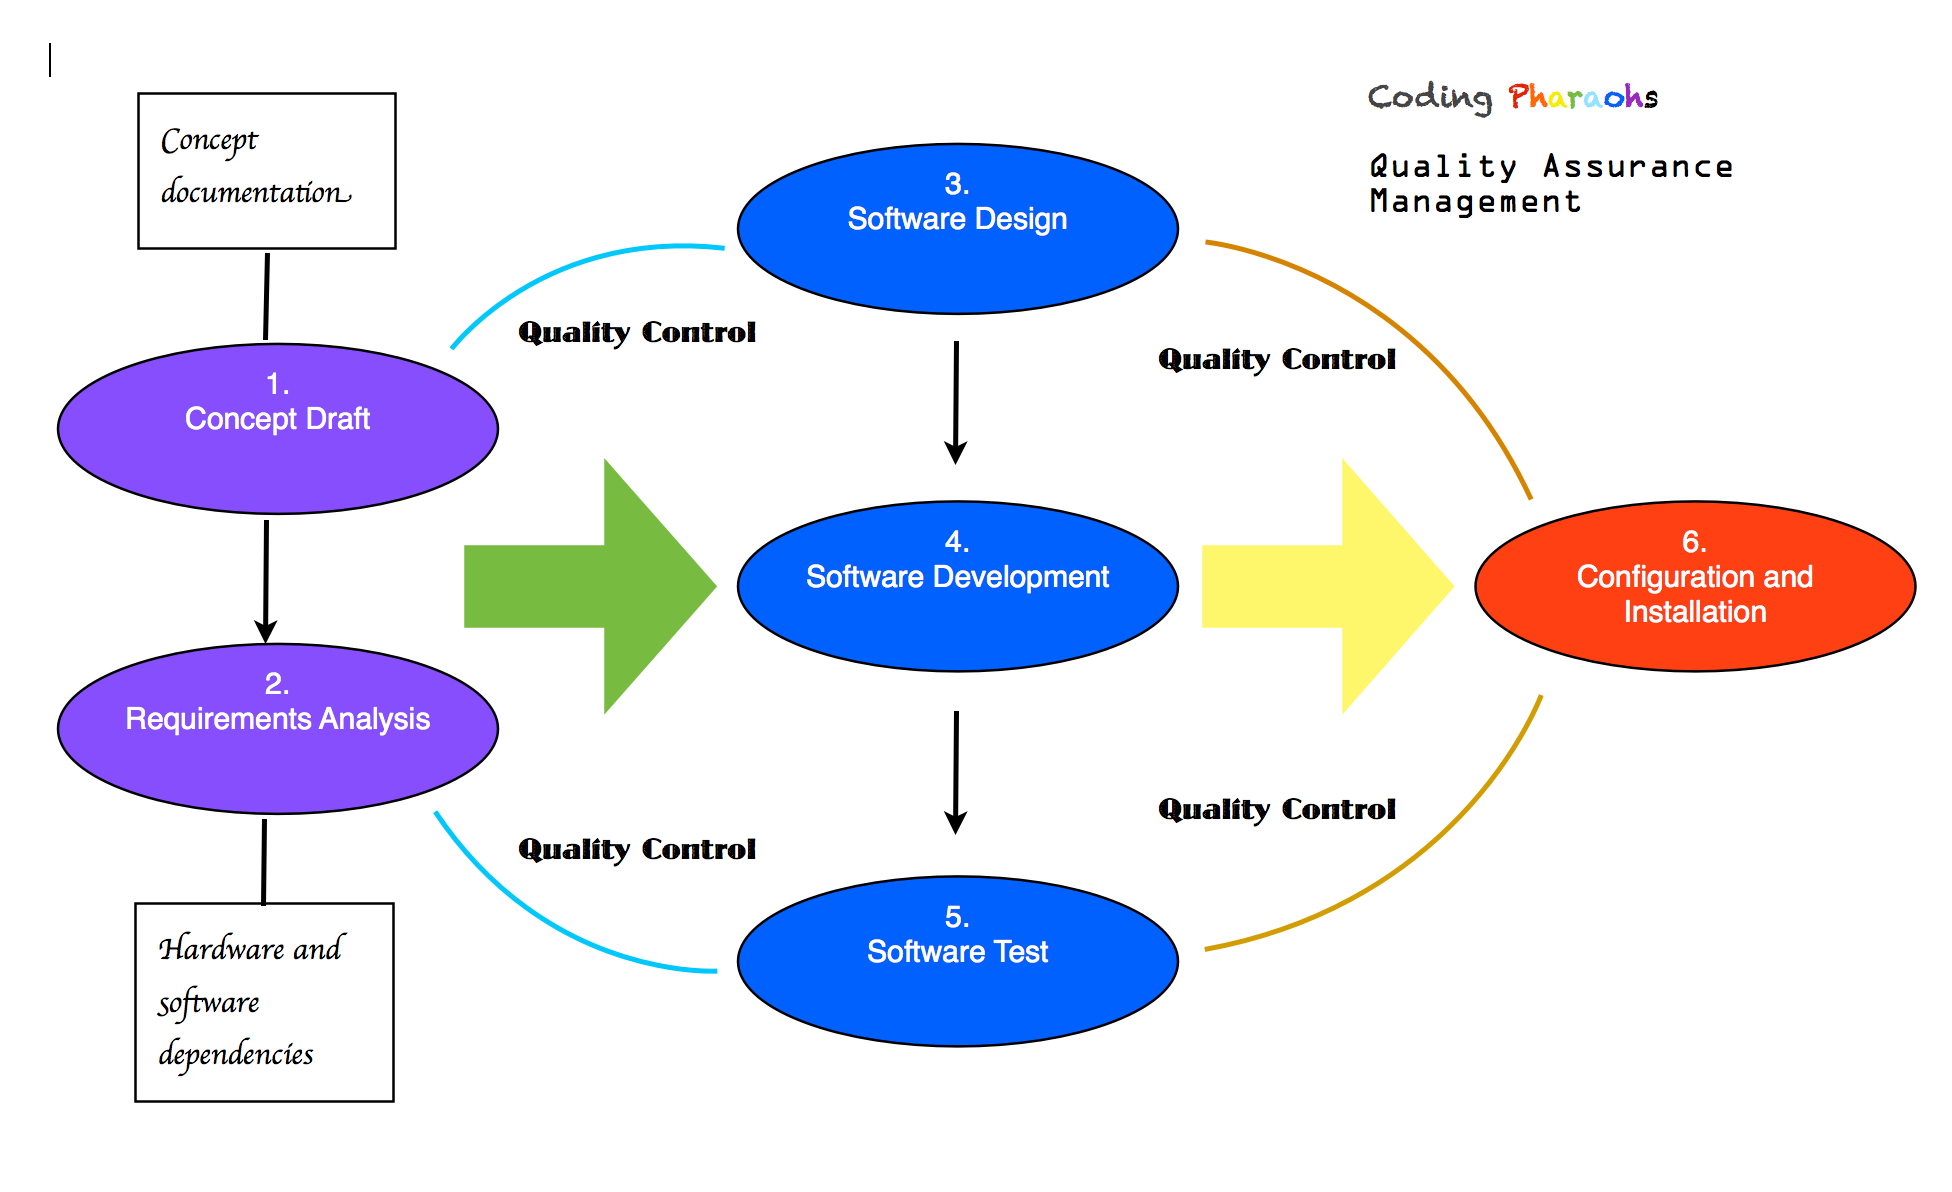
\includegraphics[width=14cm]{images/QA.png}
\end{center}
\begin{center}
\item {Diagram 3: Quality Assurance plan}
\end{center}
Quality Assurance Plan provides a guideline to the software developer as a process tool for deliverables quality assessment. It addresses the development life cycle for the group to satisfy the established SRS. 

\subsection{Verification \& Validation Process}
\subsubsection{One more thing}
The PMBOK guide is defined as follows in its 4th edition:
"Validation. The assurance that a product, service, or system meets the needs of the customer and other identified stakeholders. It often involves acceptance and suitability with external customers. Contrast with verification."\\
"Verification. The evaluation of whether or not a product, service, or system complies with a regulation, requirement, specification, or imposed condition. It is often an internal process. Contrast with validation."
\subsection{Verification \& Validation Procedures}
\newpage
\rowcolors{1}{lightgray}{white}
\begin{center}
\begin{tabular}{p{4.0cm} |p{3.5cm}|p{5cm} |}
\hline
Phase & Tasks&Key Issues \\
1.Concept Draft & Conceptual documentation	& Absorbing and understanding user's demands and discussing the constrains of implementation.\\
2. Requirements analysis and evaluation & & Analysing requirements and evaluate feasibility\\
3. Software Design & 1. Maintainability: Coding convention and documentation \newline
2. Safety evaluation \newline
3. Design analysis \newline
4. Interface design \newline
5. Stress analysis \newline
6. Test design \newline
1. & Make a rule for coding and commentating.\newline
2. Evaluating potential risk in the robot project.\newline
3. Design architecture of the robot project based on analysed requirement.\newline
4. The interface correctness, reliability and completeness in terms of hardware, software and user.\newline
5. Analysis the extreme situation in the robot project\newline
6. Design test cases \\
4. Developing 
&1. Coding based on analysis and design above\newline
2. Run functional and component tests\newline
 &1. Ensure the quality of the codes and member contribution.\newline
2. Submit test cases with results.\newline \\
5. Test & 1. Run integration test\newline
2. Run regression test\newline
3. Run stress test\newline
4. Run final test\newline
&  1. Submit the test cases with results.\newline
2.Submit the test cases with results.\newline
3. Submit the test cases with results.\newline
4. Ensure all bugs are fixed and the stability of the whole program\\
6. Configuration
&1. Configurable auditing\newline
2. V\&V final report\newline 
3. Test report


 
\end{tabular}
\end{center}
\begin{center}
\item {Table: V\&V Procedure}
\end{center}
\newpage


\section{Attachment: QA Check-list}
\subsection{Objective}

To check the quality of software development in different phases which contain the V\&V processes. This check-list will provide a intuitionistic feedback in terms of the software development, using by the score of the validation questions:\\

\subsection{Structure \& Assessment}

The document will be used to perform the checkout of quality, but considering the time allowed for the project, we will just hold the assessment twice.  
The first assessment date will be between the mid-break (21st Sep 2013 - 7th Oct 2013) and the second one will be held on Week 12 (28th Oct 2013 to 1 Nov 2013), which will be before the final presentation. Specific date will be negotiated by the group members within the period.\\
The evaluation way is defined: If Y is ticked then the marks will be increased by 1 whist N is ticked then the marks will be increased by 0. And if NA is ticked then the marks will be increased by -1.\\
The higher marks we get, the higher quality of the software development. 
\newline
   




\newpage
\subsection{Concept and Draft}
Date Performed: 
\\Performed by: 
\\Comments:
\begin{center}
\rowcolors{1}{lightgray}{white}

    \begin{tabular}{p{0.5cm} |  p{3.5cm} |  p{0.5cm} |p{0.5cm} |p{0.5cm} | p{5cm} |}
    \hline

    Item No.& Validation Item &Y &N &NA & Comment \\ \hline\hline
	3.1 &
	Does all group member understand the requirement which is proposed by the client?&
	$\text{\rlap{}}\square$& 
	$\text{\rlap{}}\square$&
	$\text{\rlap{}}\square$&
 \\ \hline


    3.2 &
	Is the requirements possible to translate into code?&
	$\text{\rlap{}}\square$& 
	$\text{\rlap{}}\square$&
	$\text{\rlap{}}\square$& \\ \hline


    3.3& 
	Has the requirements been recorded and translated into the document?&
	$\text{\rlap{}}\square$& 
	$\text{\rlap{}}\square$&
	$\text{\rlap{}}\square$& 
	\\ \hline


    3.4 &
	Has the development used a software model and software processes?&
	$\text{\rlap{}}\square$& 
	$\text{\rlap{}}\square$&
	$\text{\rlap{}}\square$& \\ \hline
	
    \end{tabular}
\end{center}



\newpage


\subsection{Requirement Analysis and Evaluation}
Date Performed:
\\Performed by:
\\Comments:

\begin{center}
\rowcolors{1}{lightgray}{white}

    \begin{tabular}{p{0.5cm} |  p{3.5cm} |  p{0.5cm} |p{0.5cm} |p{0.5cm} | p{5cm} |}
    \hline
	Item No.& Validation Item &Y &N &NA & Comment \\ \hline\hline

    	4.1 &
	Does the SRS has a clear structure so that the client could be easy to understand?&
	$\text{\rlap{}}\square$&
	$\text{\rlap{}}\square$&
	$\text{\rlap{}}\square$& \\ \hline

    4.2& 
	Has the SRS been presented to the client?&
	$\text{\rlap{}}\square$&
	$\text{\rlap{}}\square$&
	$\text{\rlap{}}\square$& \\ \hline

    4.3 &
	Has the group discussed with the client when there are changes in SRS?&
	$\text{\rlap{}}\square$&
	$\text{\rlap{}}\square$&
	$\text{\rlap{}}\square$& \\ \hline
	

    4.4 &
	Have the changes of requirements been documented in SRS?&
	$\text{\rlap{}}\square$&
	$\text{\rlap{}}\square$&
	$\text{\rlap{}}\square$& \\ \hline

    4.5&
	Have the tasks been allocated and explained clearly to the group members?&
	$\text{\rlap{}}\square$&
	$\text{\rlap{}}\square$&
	$\text{\rlap{}}\square$& \\ \hline

    4.6&
	Has the group evaluate the risk of the whole project?&
	$\text{\rlap{}}\square$&
	$\text{\rlap{}}\square$&
	$\text{\rlap{}}\square$& \\ \hline
    \end{tabular}
\end{center}





\newpage
\subsection{Software Design}
Date Performed:
\\Performed by:



\begin{center}
\rowcolors{1}{lightgray}{white}

    \begin{tabular}{p{0.5cm} |  p{3.5cm} |  p{0.5cm} |p{0.5cm} |p{0.5cm} | p{5cm} |}
    \hline
	Item No.& Validation Item &Y &N &NA & Comment \\ \hline\hline
	

    5.1&
	Has the precautions been taken to prevent the chaos of the data type?&
	$\text{\rlap{}}\square$&
	$\text{\rlap{}}\square$&
	$\text{\rlap{}}\square$& \\ \hline

    5.2&
	Has a safety analysis been adopted in the design?&
	$\text{\rlap{}}\square$&
	$\text{\rlap{}}\square$&
	$\text{\rlap{}}\square$& \\ \hline

    5.3&
	Has the system design been presented clearly to the group member?&
	$\text{\rlap{}}\square$&
	$\text{\rlap{}}\square$&
	$\text{\rlap{}}\square$& \\ \hline
 

    5.4&
	Has hardware limitation been taken account of when the system designs?&
	$\text{\rlap{}}\square$&
	$\text{\rlap{}}\square$&
	$\text{\rlap{}}\square$& \\ \hline
 

    5.5&
	Have the majority of potential risks been avoided by the design?&
	$\text{\rlap{}}\square$&
	$\text{\rlap{}}\square$&
	$\text{\rlap{}}\square$& \\ \hline
 

    5.6&
	Have the code convention, developing tools and testing tools been unified?&
	$\text{\rlap{}}\square$&
	$\text{\rlap{}}\square$&
	$\text{\rlap{}}\square$& \\ \hline


 


 
    \end{tabular}
\end{center}



\newpage
\subsection{Developing}
Date Performed:
\\Performed by:


\begin{center}
\rowcolors{1}{lightgray}{white}

    \begin{tabular}{p{0.5cm} |  p{3.5cm} |  p{0.5cm} |p{0.5cm} |p{0.5cm} | p{5cm} |}
    \hline
	Item No.& Validation Item &Y &N &NA & Comment \\ \hline\hline
	

    6.1&
	Have special/additional requirements been documented?& 
	$\text{\rlap{}}\square$&  
	$\text{\rlap{}}\square$&
	$\text{\rlap{}}\square$& 
	\\ \hline

    6.2&
	Does all code have adequate comments so that it is easy to read by each member in the group?&
	$\text{\rlap{}}\square$&
	$\text{\rlap{}}\square$&
	$\text{\rlap{}}\square$& 
	\\ \hline

    6.3&
	Has the code review session been held?&
	$\text{\rlap{}}\square$&
	$\text{\rlap{}}\square$&
	$\text{\rlap{}}\square$&
\\ \hline

    6.4&
	Have all group members clearly know the code tasks?&
	$\text{\rlap{}}\square$&
	$\text{\rlap{}}\square$&
	$\text{\rlap{}}\square$& 
	\\ \hline

    6.5&
	Does each function have its own succinct description?&
	$\text{\rlap{}}\square$&
	$\text{\rlap{}}\square$&
	$\text{\rlap{}}\square$& 
	\\ \hline

    6.6&
	Have the white-box tests been created and reported the results to the test manager?&
	$\text{\rlap{}}\square$&
	$\text{\rlap{}}\square$&
	$\text{\rlap{}}\square$& 
	\\ \hline

    6.7&
	Did the whole program pass all functional and component tests?&
	$\text{\rlap{}}\square$&
	$\text{\rlap{}}\square$&
	$\text{\rlap{}}\square$& 
	\\ 
	\hline

    6.8&
	Has test report included all the test results?&
	$\text{\rlap{}}\square$&
	$\text{\rlap{}}\square$&
	$\text{\rlap{}}\square$& 
	\\ \hline
	
 	6.9&
	Has the client been told when the SRS has been updated?&
	$\text{\rlap{}}\square$&
	$\text{\rlap{}}\square$&
	$\text{\rlap{}}\square$& 
	\\ \hline

   
    \end{tabular}
\end{center}



\newpage
\subsection{Testing}
Date Performed:
\\Performed by:



\begin{center}
\rowcolors{1}{lightgray}{white}

    \begin{tabular}{p{0.5cm} |  p{3.5cm} |  p{0.5cm} |p{0.5cm} |p{0.5cm} | p{5cm} |}
    \hline
	Item No.& Validation Item &Y &N &NA & Comment \\ \hline\hline
	

    7.1&
	Is there any mirror bug affecting the whole program?&
	$\text{\rlap{}}\square$&
	$\text{\rlap{}}\square$&
	$\text{\rlap{}}\square$& \\ \hline

    7.2&
	Are the error messages kept independently?&
	$\text{\rlap{}}\square$&
	$\text{\rlap{}}\square$&
	$\text{\rlap{}}\square$& \\ \hline

    7.3&
	Are all errors during the testing been recorded?&
	$\text{\rlap{}}\square$&
	$\text{\rlap{}}\square$&
	$\text{\rlap{}}\square$& \\ \hline
 

    7.4&
	Did the whole program pass all integration tests?&
	$\text{\rlap{}}\square$&
	$\text{\rlap{}}\square$&
	$\text{\rlap{}}\square$& \\ \hline
  

    7.5&
	Did the whole program pass all regression and stress tests?&
	$\text{\rlap{}}\square$&
	$\text{\rlap{}}\square$&
	$\text{\rlap{}}\square$& \\ \hline
  

    7.6&
	Did the whole program pass final test?&
	$\text{\rlap{}}\square$&
	$\text{\rlap{}}\square$&
	$\text{\rlap{}}\square$& \\ \hline
   
 
    \end{tabular}
\end{center}

\end{document}
